\documentclass[]{article}

\usepackage[ngerman]{babel}
\usepackage{hyperref}
\usepackage{amsmath}

%opening
\title{Building an oscilloscope using RP Pico to measure an LC-Circuit}
\author{Len-Marvin Adler, Deniz}

\begin{document}

\maketitle
\clearpage
\tableofcontents
\clearpage

%% content of sections is written in the included files
%% 1.
\section{Einleitung}

Ein Oszilloskop ist ein Messgerät, dass in seiner Grundfunktion Spannungen
über einen Zeitverlauf lang messen und darstellen kann. \newline
Diese Darstellung erfolgt auf einem Display \cite{KnowUrOscilloscope}. \newline
%\begin{figure}[htpb]
%	\centering
%	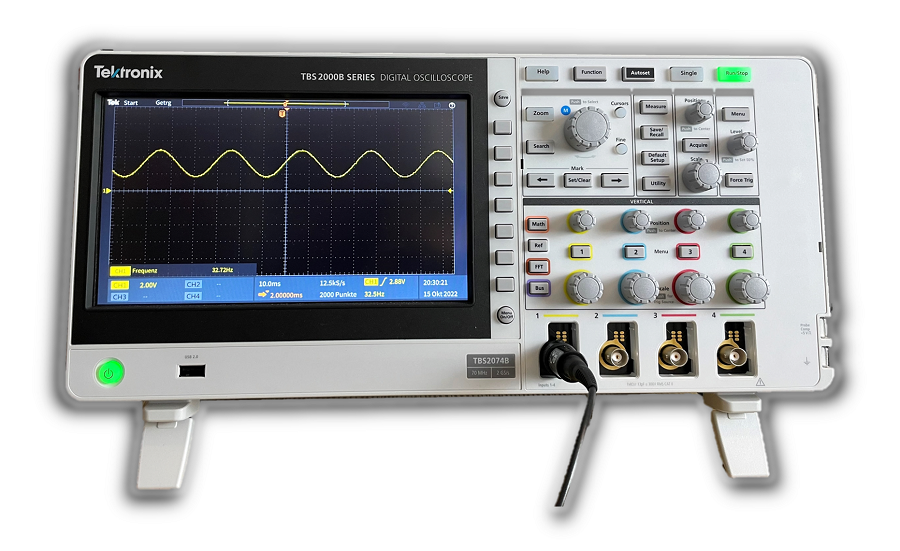
\includegraphics[width=\textwidth,height=6cm,keepaspectratio=true]{images/OszilloskopBeispiel.png}
%	\caption{
%		Oszilloskop aus \cite{OscilloscopeBild}
%	}
%	\label{Label}
%\end{figure} \newline
Komplexere Oszilloskope können häufig auch Messwerte persistent speichern oder die Skalierung der Achsen
ändern. Wegen letzterem lässt sich ein großer Umfang von Spannungswerten messen.
Durch diese Funktionen ist das Oszilloskop ein oft- und vielseitig verwendetes Messgerät
in der Elektrotechnik \cite{ETechnikEinfach}. \newline \newline
In dieser Seminararbeit wollen wir unser eigenes Oszilloskop bauen, das die Grundfunktionen,
eine Zeit lang Spannungen  zu messen und darzustellen, erfüllen soll.
Hierfür werden zuerst die groben Komponenten und deren Zusammenspiel im selbstgebauten Oszilloskop erläutert.\newline
Danach wird auf die einzelnen Bauteile und ihre Funktion eingegangen und
zuletzt eine Messung eines einfachen Schwingkreises durchgeführt, um an diesen Messwerten zu begründen,
ob das Oszilloskop die Anforderungen erfüllt.  



%% 2.
\section{Vorraussetzungen}
\label{Vorraussetzungen}

%% What you need for building our oscilloscope
%% also reasoning for the devices

\subsection{Geräte}




\subsection{Zusammenspiel}

Alle Geräte zusammen sehen als Schaltplan so aus:
\begin{figure}[h]
	\centering
	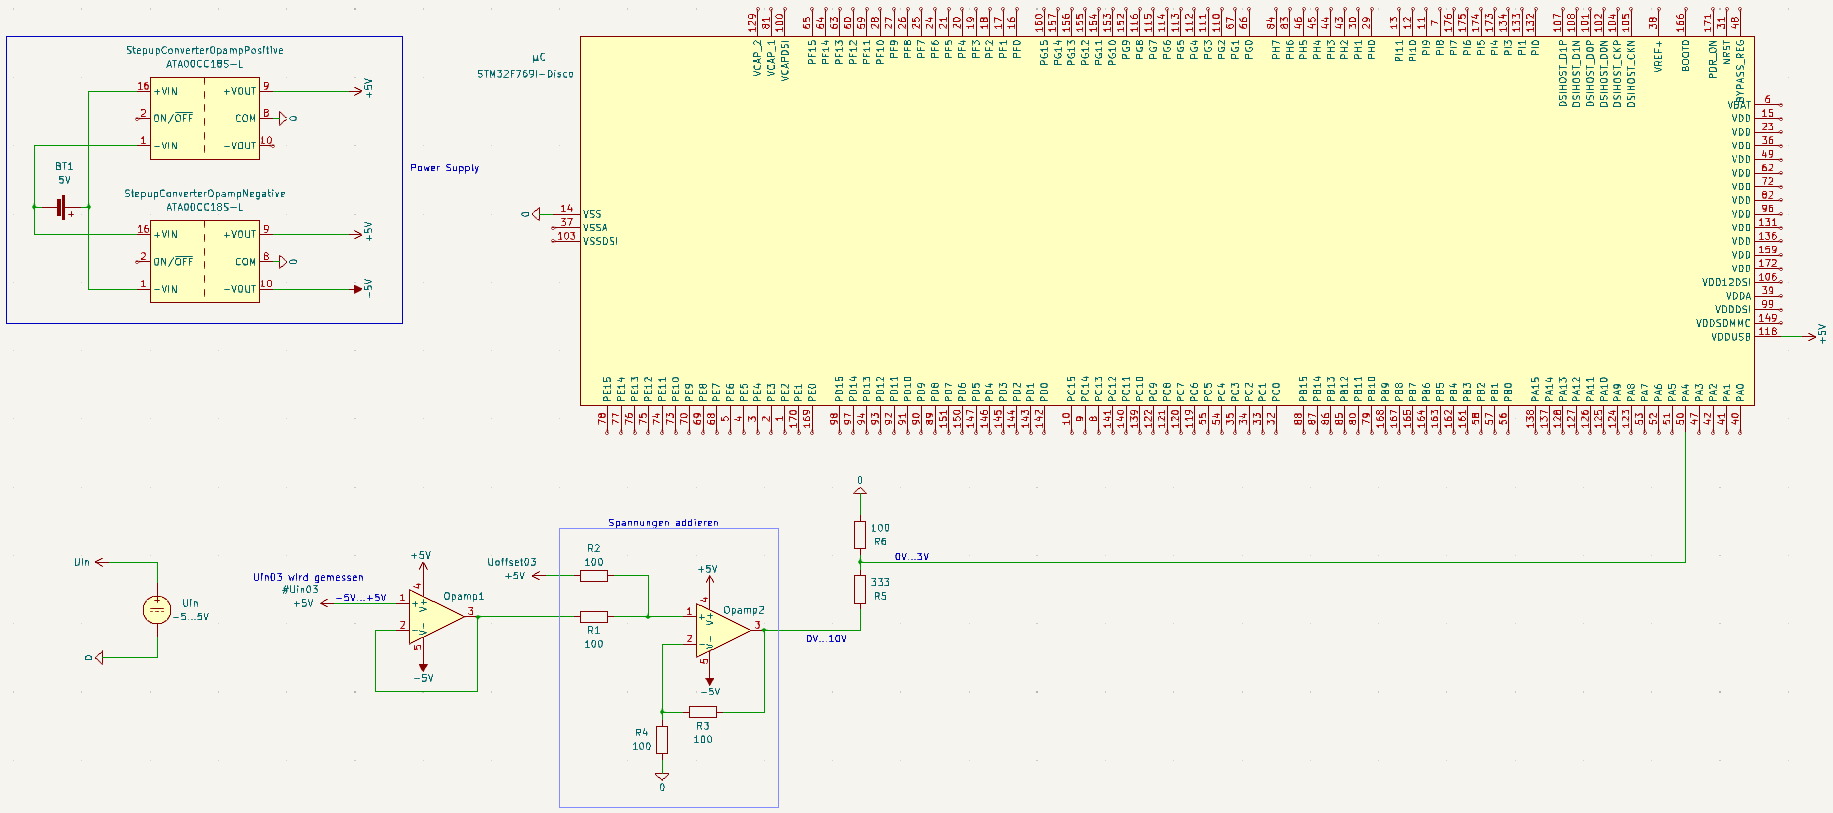
\includegraphics[width=\textwidth, scale=0.5]{images/schematic_opamps2.png}
	\caption{Schematischer Aufbau des Oszilloskops}
\end{figure}


Oszilloskop Eingang ist $U_{in}$ und der Ground $0$. \newline
Für die Messung, muss das Oszilloskop zur gemessenen Spannung parallel geschalten werden,
damit die Spannung am Oszilloskop die gleiche ist, wie die am gemessenen Stromkreis.

\subsubsection{Idee}
Die Eingangsspannung $U_{in}$ liegt im Intervall $[-15, 15] V$,
der GPIO Pin des Mikrocontrollers erlaubt allerdings nur $[0, 3.3] V$. \newline
Folglich muss die Eingangsspannung dahingehend bereinigt werden.
\newline \newline
Hierfür bringen wir die Eingangsspannung erstmal in den positiven Bereich, indem wir
eine Offset Spannung $U_{offset} = 15V$, mithilfe eines Nicht-invertierten Summerverstärkers, erläutert in \ref{Addition einer Offset-Spannung}, dazu addieren. \newline
Der Spannungsbereich ändert sich dadurch zu $[0, 30] V$.
Dieser muss nun lediglich, mithilfe eines Spannungsteilers, siehe \ref{Spannungsteiler}, zu $[0, 3.3] V$ aufgeteilt werden.
Damit der gemessene Stromkreis durch das Oszilloskop nicht belastet wird, muss noch ein Bauteil mit einer hohen Eingangsimpedanz, erläutert in \ref{Unbelastete Eingangsspannung}, vor das ganze Netzwerk geschalten werden.


\subsubsection{Stromversorgung}
Der Mikrocontroller wird über USB mit $5V$ versorgt.
Die beiden Opamps werden durch eine Batterie mithilfe von Stepup Convertern versorgt.

Später werden die einzelnen Schritte ausführlicher erläutert und begründet.





%% 3.
\section{Eingangsspannung bereinigen}
\label{Eingangsspannung bereinigen}

%% Describes our Opamps and Voltage divider
%% also reasoning for choosing those specific
%% values of resistor, power supply, etc.
Der GPIO Pin aus \ref{Mikrocontroller}, an dem die Spannung mithilfe eines Mikrocontrollers gemessen wird,
kann nur Spannung im Bereich $[0, 3.3]V$ messen.
Das Oszilloskop soll allerdings einen größeren Spannungsbereich $[-5, 5]V$ messen können.
Daher wird nun die Eingangsspannung bereinigt, sodass sie den Anforderungen des GPIO Pin genügt.

\subsection{Unbelastete Eingangsspannung}
\label{Unbelastete Eingangsspannung}
Der Stromkreis, der gemessen wird, soll nicht belastet werden, daher wird ein Opamp mit
hoher Eingangsimpedanz und einem Verstärkungsfaktor von $1$ benutzt.
Dies wird durch eine Rückkopplung des Ausgangs an den invertierten Eingang des Opamps erreicht.
\begin{figure}[h]
	\centering
	\includegraphics[width=0.7\textwidth]{images/schematic\_teil1\_unbelastet\_opamp.png}
	\caption{Schaltplan um den Eingangsstrom nicht zu belasten, Ausschnitt aus \ref{Gesamte_Schematic}}
\end{figure}


\subsection{Addition einer Offset-Spannung}
\label{Addition einer Offset-Spannung}

Nun gilt es den Spannungsbereich von $[-5, 5]V$ auf $[0, 10]V$ zu legen.
Dafür wird eine Offset-Spannung $U_{offset}$, die aus einem $V_{CC}$ Pin
des Mikrocontrollers stammt und mithilfe des Stepup Spannungsreglers auf $5V$ gebracht wird, zur Eingangsspannung dazu addiert.
Dies geschieht mit einem Nichtinvertierenden Summierverstärker, also ein Opamp der extern mit
Spannungsteilern, gemäß \autoref{fig:Opamp_Adder}, beschalten ist.
Der Opamp arbeitet also mit Spannungen im Bereich $[-5,10]V$,
daher muss der Bereich der Versorgungsspannung mindestens diese Spannungswerte enthalten.
Experimentell hat sich herausgestellt, dass der \textit{TS912IN} funktioniert, solange die Eingangsspannung
unterhalb von $1.7V$ der Versorgungsspannung liegt.
Daher wird für den Opamp großzügig eine positive Versorgungsspannung von $V^+_{CC} = 15V$ und eine 
negative von $V^-_{CC} = -15V$ gewählt.
Für die maximale Eingangsspannung gilt $\max(U_{in}) + U_{offset} = 5V + 5V = 10V < (15V - 1.7V)$
und für die minimale gilt $\min(U_{in}) + U_{offset} = -5V + 5V = 0V$.
Der Opamp funktioniert also für die definierte Eingangs- und Offsetspannung. \newline
Es gilt, laut \cite{Opamp_adder}, für die Ausgangsspannung $U_3$ des Opamps:
\begin{align*}
U_3 &= (U_{in} \cdot \frac{R_2}{R_1 + R_2} + U_{offset} \cdot \frac{R_1}{R_1 + R_2}) \cdot(1 + \frac{R_4}{R_3}) \\
	&= (U_{in} \cdot \frac{1}{2} + U_{offset} \cdot \frac{1}{2}) \cdot 2 \\
	&= U_{in} + U_{offset}
\end{align*}

\begin{figure}[h!]
	\centering
	\includegraphics[width=0.7\textwidth]{images/schematic\_teil2\_adder.png}
	\caption{Addition von $U_{in}$ und $U_{offset}$, Ausschnitt aus \ref{Gesamte_Schematic}}
	\label{fig:Opamp_Adder}
\end{figure}

%Eine Messung der Spannung von $U_{in}$ und $U_3$ mittels eines kommerziellen Oszilloskops zeigt,
%für eine Wechselspannung mit Amplitude $5V$, erfolgreich $U_3 = U_{in} + U_{offset}$:
%\begin{figure}[h!]
%	\centering
%	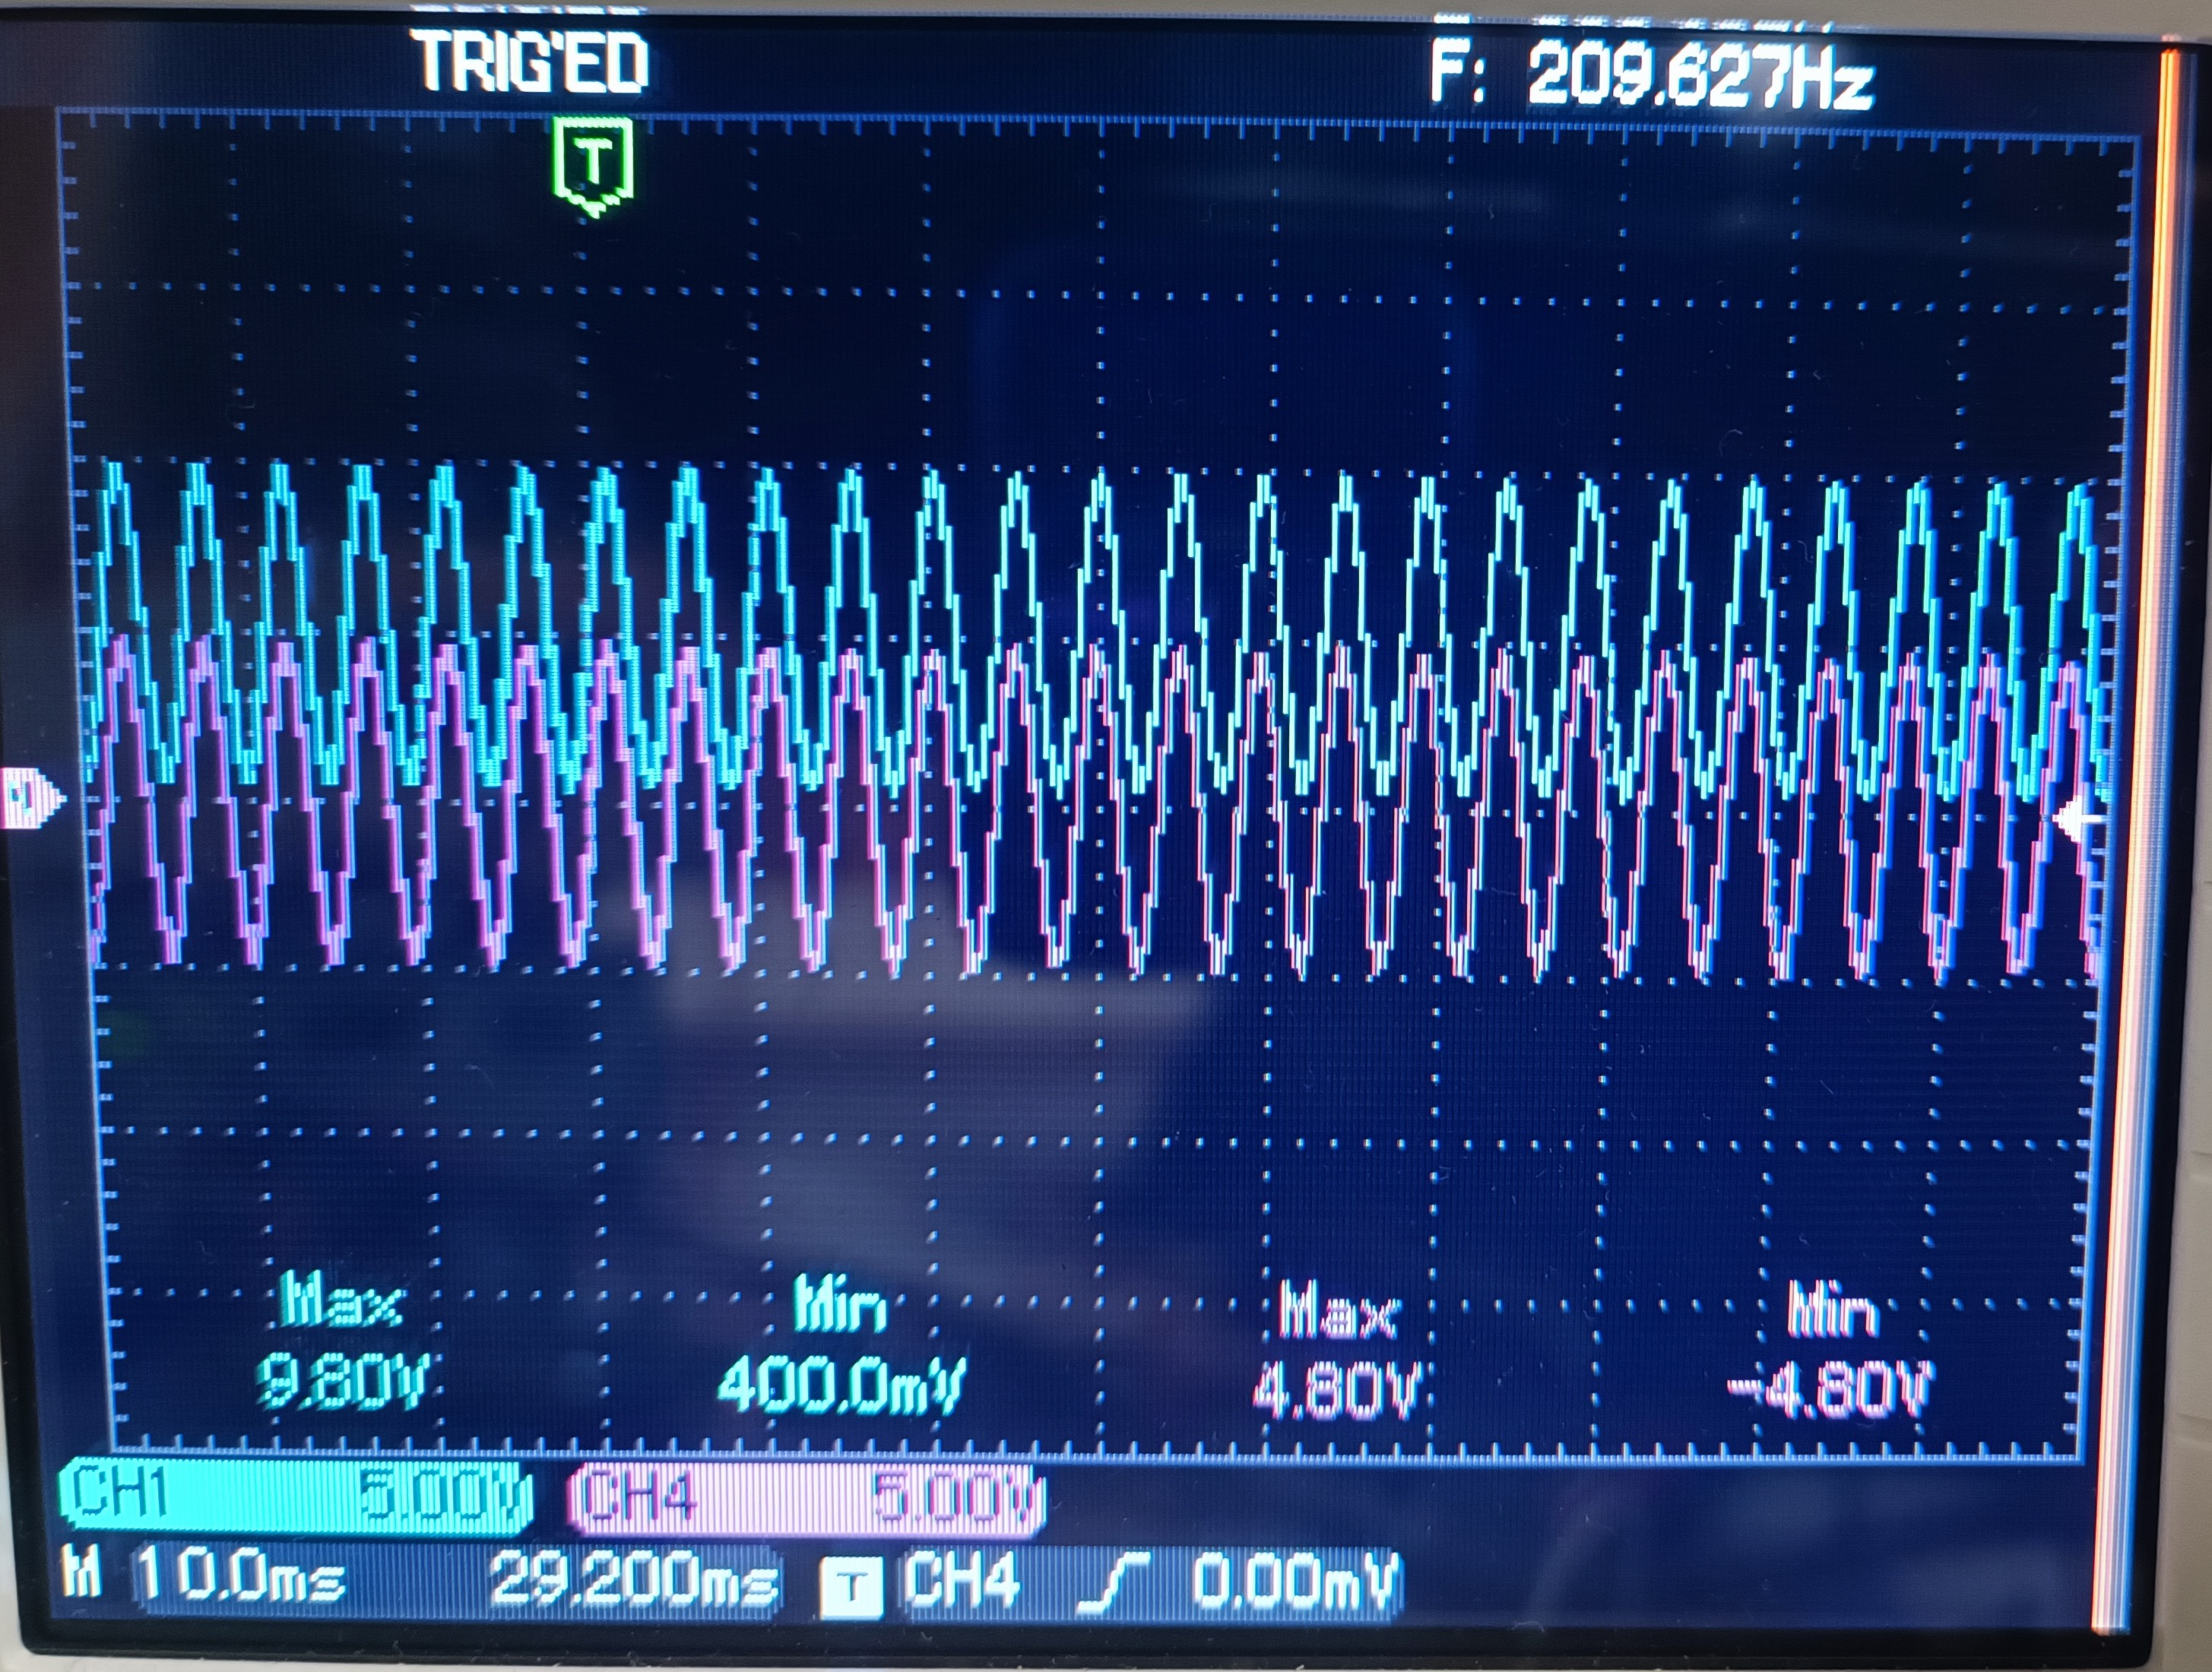
\includegraphics[width=0.7\textwidth]{images/messung_adder.jpg}
%	\caption{Messung von $U_{in}$ (lila) und $U_3$ (blau)}
%\end{figure}

\subsection{Spannungsteiler}
\label{Spannungsteiler}

Zuletzt wird die Spannung $U_3$, welche aus \textit{Opamp2} gegeben wird, geteilt, sodass
sie im Bereich $[0, 3.3]V$ für den GPIO Pin liegt.
Der Spannungsteiler $(R_5, R_6)$ teilt $U_3$ dabei zu
$U_{GPIO} = U_3 \cdot \frac{R_6}{(R_5 + R_7) + R_6} = U_3 \cdot \frac{100 \Omega}{330 \Omega}$. \newline
Dadurch ergibt sich ein Spannungsbereich für $U_{GPIO}$ von
$[0, 10 \cdot \frac{100}{330}]V = [0, 3.3]V$.
\begin{figure}[h!]
	\centering
	\includegraphics[scale=0.7]{images/schematic\_teil3\_spannungsteiler.png}
	\caption{Spannungsteiler zu $U_{GPIO}$, Ausschnitt aus \ref{Gesamte_Schematic}}
\end{figure}
\newline
Die bereinigte Spannung $U_{GPIO}$ wird nun an den GPIO Pin des Mikrocontrollers angeschlossen.





%% 4.
\section{Raspberry Pi Pico}

%% Describes Pico, GPIO, registers, etc.
%% also some internal processing values
%% e.g. Taktrate am GPIO,
%%      Genauigkeit beim messen am GPIO
Pico

\subsection{GPIO}


\subsection{Register}


\subsection{ADC}

ADC

\subsubsection{Lineare Funktion}
The ADC defines a linear map 
$$f: [0,3.3] \rightarrow [\texttt{0x0}, \texttt{0xFFF}]$$ \newline
\texttt{0xFFF} because 12 bit register. \newline
TODO: Prove that this is a function... \newline
This function takes an analog input (voltage at GPIO) and writes the corresponding value into the GPIO register. \newline
This \texttt{Hex} value is not the value of the actual voltage, only a mapping, though.
TODO: Prove that an inverse exists... \newline
To calculate the measured voltage we define an inverse
$$
	f^{-1}: [\texttt{0x0}, \texttt{0xFFF}] \rightarrow [0, 3.3]
$$


%% 5.
\section{Beispiel-Nutzung}

%% describes an exampe of Usage
%% schaltkreis, messwerte, etc.
%% von Schwingkreis (LC-Circuit)
Example

\subsection{Schwingkreis}


%% 6.
\section{Benchmarking}

\subsection{Messaufbau}
Wie wird unser Oszilloskop gebenchmarked

\subsection{Messdurchführung}

Wie wird die Messung mit Oszilloskop durchgeführt

\subsection{Messwerte}

Was für quantitative Werte gemessen wurden

\subsection{Auswertung}

Was das für unser Oszilloskop bedeutet



%% Benchmarking our oscilloscope
%% vs. a real/professional one
%% Taktrate, Genauigkeit, etc.


%% 7.
\section{Diskussion}

%% issues we faced or
%% issues oscilloscope has (maybe already in 6-Benchmarking)
Issues


%% 8.
\section{Fazit}

%% Schlusswort / final words
Das Oszilloskop misst akzeptabel gut im Bereich der Anforderungen, daher
kann es für Messungen in diesem Bereich eingesetzt werden.
Jedoch steht es einem kommerziellen Oszilloskopen im Triggering, Darstellungsbereich der Messung und 
in der Messfrequenz nach.
Es wird daher angeraten, es nicht für professionelle Messungen zu verwenden.
Für Hobbyprojekte, beziehungsweise um eine simple Spannungskurve zu sehen,
sollte das Oszilloskop dennoch ausreichen und man muss kein kommerzielles Gerät kaufen.


%% Bibliography
\bibliographystyle{plain}
\bibliography{bib/bibliography.bib}

\end{document}
